\documentclass{article}

\usepackage{amsmath}
\usepackage{authblk}
\usepackage[margin=1in]{geometry}
\usepackage{graphicx} % Required for inserting images

\title{Swinging, Fast and Slow: Untangling intention and timing error from bat speed and swing length in Major League Baseball}
\date{}
\author[1]{Scott Powers}
\author[2]{Ronald Yurko}
\affil[1]{Department of Sport Management, Rice University}
\affil[2]{Department of Statistics \& Data Science, Carnegie Mellon University}

\begin{document}

\maketitle

\subsection*{Introduction}

In May 2024, Major League Baseball (MLB) released a novel dataset of pitch-level swing tracking metrics. The data are limited to bat speed and swing length at contact point, with a teaser of more to come.

Interpretation of bat speed and swing length is complicated by the measurement point. For the exact same swing mechanics, if the batter swings later (or the ball moves faster), the contact point occurs upstream in the swing path. This results in a shorter swing length measurement and a slower bat speed measurement (because the bat accelerates up to and beyond intended contact). If the batter swings earlier (or the ball moves slower), the contact point occurs downstream in the swing path, causing a different measurement bias. Bat speed and swing length, therefore, reflect not only the swing but also the outcome of the swing.

This complication has not discouraged data scientists from making claims about what constitutes a {\it good} swing and how batters {\it should} try to swing. In the present work, we take a more cautious approach, seeking to understand and classify the sources of swing-to-swing variability in bat speed and swing length.

\subsection*{Data}

Our dataset comprises 96,887 swings by MLB players between April 3 and May 30, 2024. For each swing, we observe bat speed and swing length. {\bf Bat speed} is the linear speed of the {\it sweet spot} of the bat (approximately six inches from the end), measured at the point of contact with the ball. If no contact occurs, the contact point is defined as the point of minimum distance between ball and sweet spot. {\bf Swing length} is the distance travelled by the end of the bat from start of swing to contact point. In addition to these novel swing tracking metrics, we have ball tracking data (most notably pitch speed, pitch location and batted ball speed) and contextual data (most notably ball-strike count). All data are publicly available from Baseball Savant.

\subsection*{Methods}

\noindent {\bf Cleaning the data.}
The initial dataset includes attempted bunts (which are labelled) and attempted {\it check-swings} (i.e., partial swings, not labelled). We aim to limit our analysis to full swings. When reporting aggregate metrics like average bat speed, MLB filters out each batter's bottom 10\% of swings by bat speed, labelling the remaining swings as {\it competitive}. We take a more inclusive approach by filtering out only swings with bat speed below 50 mph (which filters out all bunt attempts). Based on video review, this cutoff does a good job of distinguishing between full and partial swings while only removing $\approx$ 2.5\% of swings.

We reproduce MLB's derived metric for {\it squared-up} contact as:
\begin{equation}
  \label{eqn:squared-up}
  \mbox{batted ball speed} > 80\% \times \left\{1.23 \cdot (\mbox{bat speed}) + 0.23 \cdot (\mbox{pitch speed})\right\}.
\end{equation}
The right-hand side of (\ref{eqn:squared-up}) is a rough approximation for 80\% of the theoretical maximum batted ball speed given bat speed and pitch speed at contact (with additional assumptions about the mass of bat and ball). In our dataset, we observe batted ball speeds as high as 110\% of the rough theoretical maximum.

~\\
\noindent {\bf Predicting swing intention.}
We begin with the hypothesis that two covariates explain real (non-artifactual) differences in swing mechanics: ball-strike count and pitch location. To the extent that a batter's swing tracking metrics co-vary with count, we describe this as their {\it approach}. To the extent that a batter's swing tracking metrics co-vary with pitch location, we describe this as swing {\it adaptation}. Acknowledging that swing timing biases the measurement of bat speed and swing length, we mitigate this confounding bias by {\bf filtering on swings that result in squared-up contact} and fit a linear mixed-effects model:
\begin{align}
    \label{eqn:intended-swing-length}
    \begin{split}
    (\mbox{swing length})_i = \alpha + \gamma^A_{b_i}
        & + (\beta^B + \gamma^B_{b_i}) \cdot (\mbox{balls})_i
          + (\beta^S + \gamma^S_{b_i}) \cdot (\mbox{strikes})_i\\
        & + (\beta^X + \gamma^X_{b_i}) \cdot (\mbox{pitch loc x})_i
          + (\beta^Z + \gamma^Z_{b_i}) \cdot (\mbox{pitch loc z})_i
          + \epsilon_i,\\
    \gamma^A_b \sim \mathcal{N}(0, \sigma^2_A), \hspace{2mm}
    \gamma^B_b \sim \mathcal{N}(0, \sigma^2_B), \hspace{2mm}
   &\gamma^S_b \sim \mathcal{N}(0, \sigma^2_S), \hspace{2mm}
    \gamma^X_b \sim \mathcal{N}(0, \sigma^2_X), \hspace{2mm}
    \gamma^Z_b \sim \mathcal{N}(0, \sigma^2_Z), \hspace{2mm}
    \epsilon_i \sim \mathcal{N}(0, \sigma^2_\epsilon),
    \end{split}
\end{align}
where $b_i$ is the batter swinging at pitch $i$. The $\gamma$ parameters are random intercepts and random slopes. We fit a model with the same specification to predict intended bat speed. These models tell us: What are the bat speed and swing length (by batter, count and pitch location) when the timing is good? We interpret the prediction from this model on each pitch as the {\it intended} bat speed and swing length.

~\\
\noindent {\bf Estimating swing timing.}
We define timing as the standard deviation of residual (observed minus intended) bat speed and swing length. This is a two-dimensional measurement with units of miles per hour and feet. We hypothesize that smaller values in both dimensions (i.e., less timing error) are better.

\subsection*{Results}

Figure 1 demonstrates the practical significance of separating the variation due to intention from the variation due to timing error. Between intended bat speed and swing length, we see an approximately linear relationship. However, we see a very different relationship between residual (observed minus intended) bat speed and swing length. This curve seems to trace the speed of the bat along the path of the swing, accelerating until shortly after the intended contact point and then slowing down. In addition, we have interpretable metrics describing each batter's approach, swing adaptation and timing (not shown in this abstract).

~\\
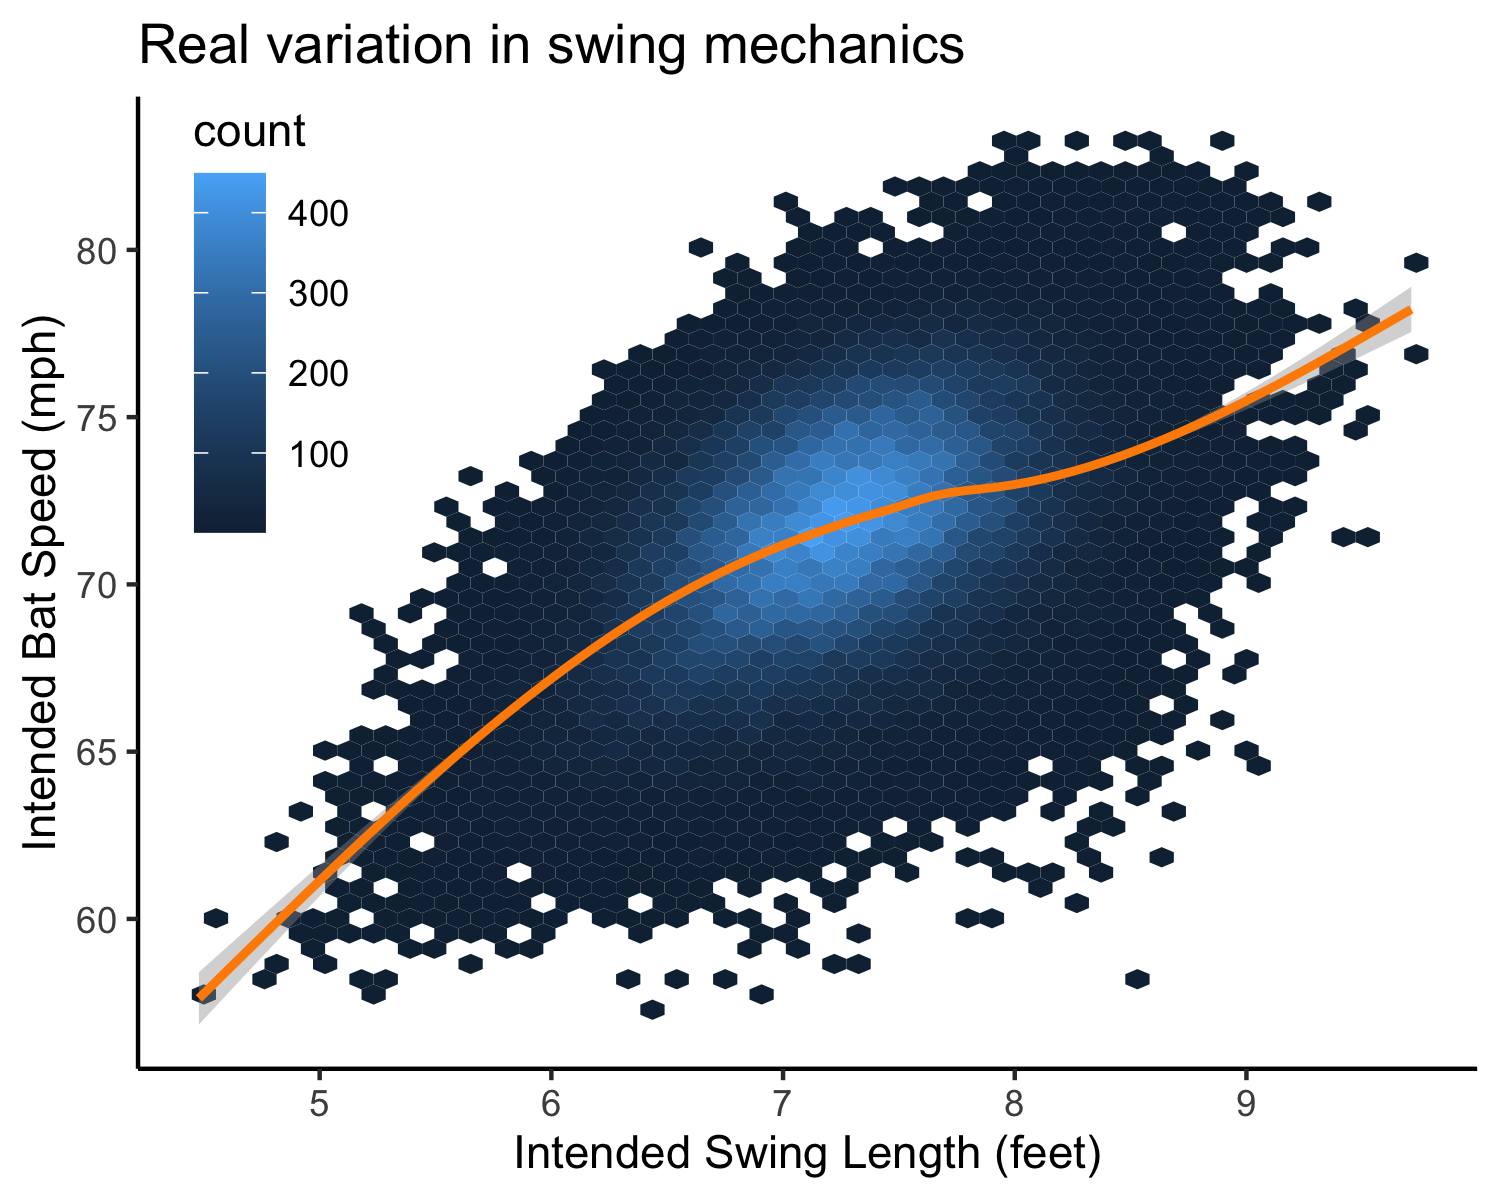
\includegraphics[width = 0.5\textwidth]{../../figures/intention.png}\hspace{4mm}
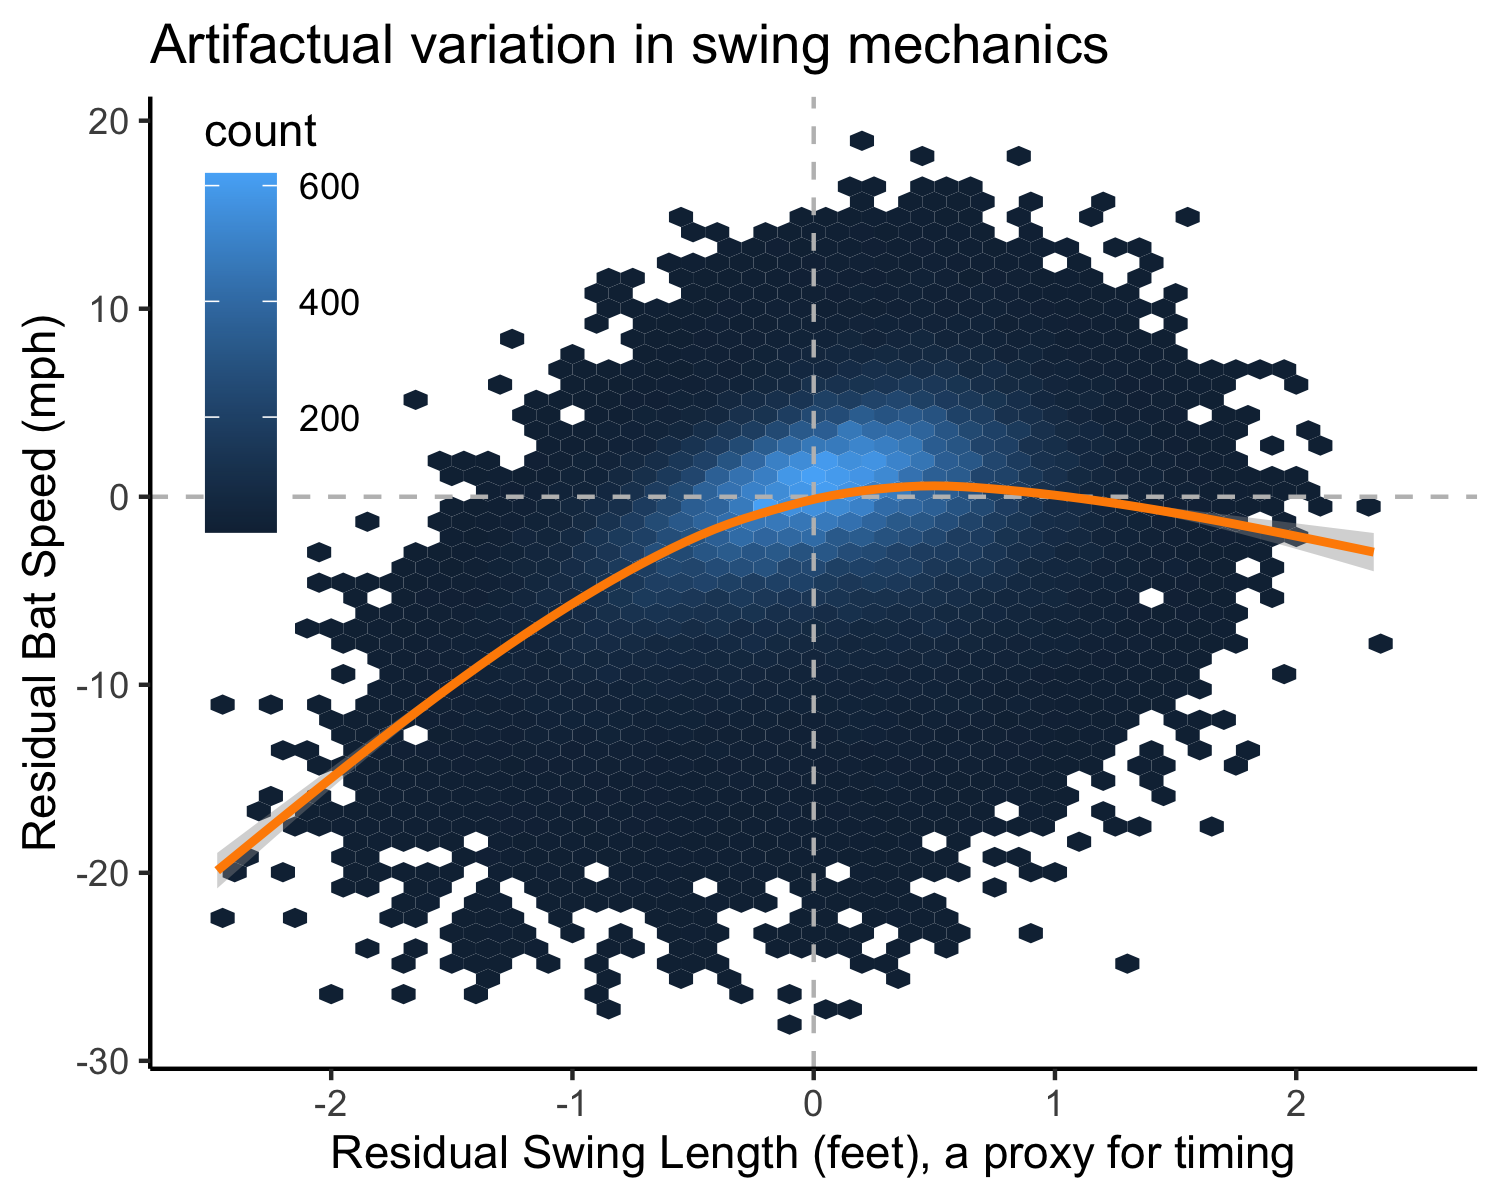
\includegraphics[width = 0.5\textwidth]{../../figures/residual.png}\\
{\it\footnotesize Figure 1. (left) Intended bat speed vs. swing length. (right) Residual (observed minus intended) bat speed vs. swing length.}

\subsection*{Conclusion}

By predicting batter intention, we mitigate the effect of timing error on measuring bat speed and swing length. It is too early to conclude that our timing metric is a valid measurement of swing timing. As Figure 1 shows, there is still much variation in residual bat speed that remains unexplained by residual swing length. These improved measurements of real (non-artifactual) variation in swing mechanics will enable future research on topics such as the effect of approach on results.

\end{document}
